\problem{}
Given an $m \times n$ matrix in which every element is a positive integer, you need to select a subset of the elements in the matrix so that these selected elements are not adjacent. We define that element $(i, j)$ is adjacent to elements $(i, j \pm 1)$ and $(i \pm 1, j)$ but is not adjacent to elements $(i \pm 1, j \pm 1)$. Design an efficient algorithm that maximizes the sum of the selected elements.

\textbf{Solution:}

This can be seen as a maximum-weight independent set problem, we can use min cut to obtain the result. First we separate the elements into a bipartite graph. That means adjacent elements belong to different set $X,Y$.
\begin{figure}[htbp]
	\begin{center}	
		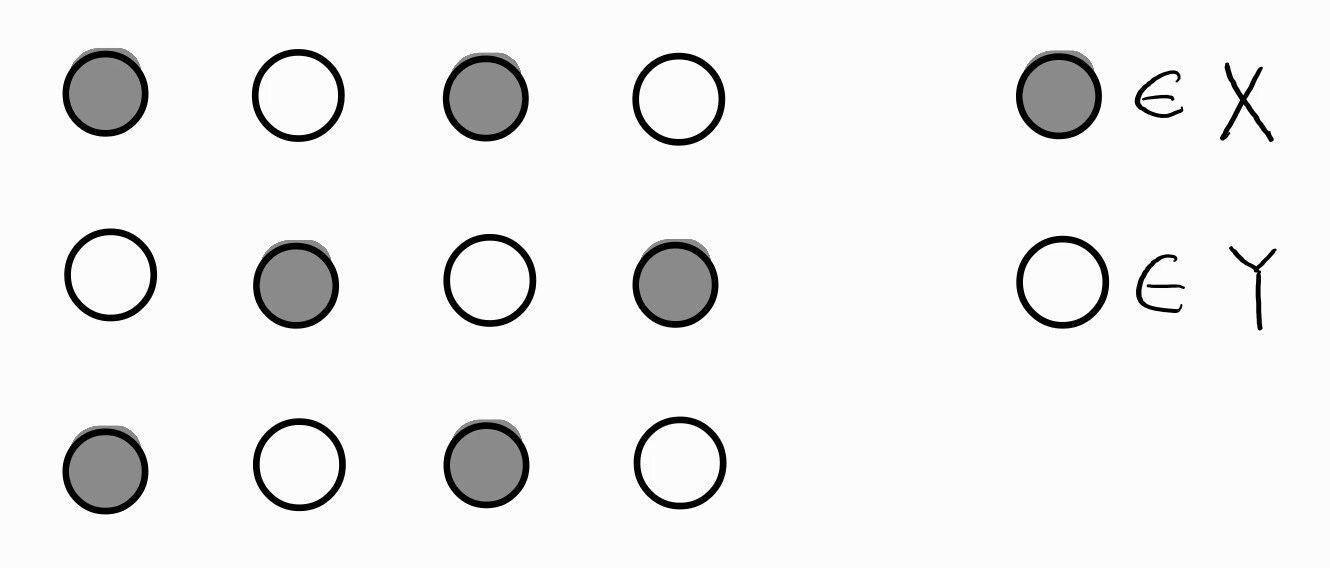
\includegraphics[width=0.4\textwidth]{HW2/1.jpg}
	\end{center}
\end{figure} 

Add $s$ and $t$. Connect a directed edge from $s$ to each vertex in the set $X$ with capacity equal to the integer of elements. Then make a directed edge from each vertex in the set $Y$ to $t$ with capacity equal to the integer of elements. Finally, adjacent elements $x_i, y_j$ are connected from $x_i$ to $y_j$ by a directed edge of $\infty$ capacity.

\begin{figure}[htbp]
	\begin{center}	
		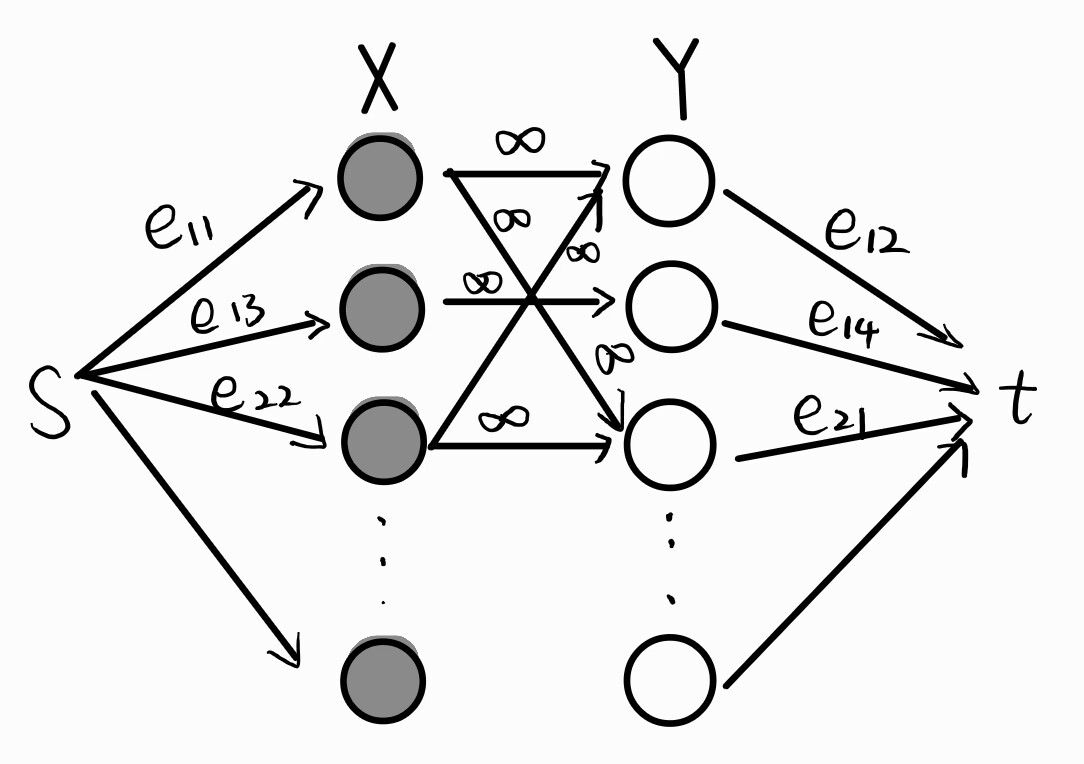
\includegraphics[width=0.4\textwidth]{HW2/2.jpg}
	\end{center}
\end{figure} 

According to "Max-flow min-cut theorem", we can directly caculate the maximum flow on the network, and the result equals to
$$Result =  \sum_{i=1}^{M}\sum_{j=1}^{N}e_{ij} - flow_{max}$$

\textbf{Analysis:}
Use Ford-Fulkerson to caculate Max-flow, so the time complexity is $O(mn)$